%! Author = Len Washington III
%! Date = 11/6/24

% Preamble
\documentclass[
	chapter=9,
	title={Basic Concepts of Chemical Bonding},
	showanswers=true,
]{chem122notes}
\usepackage{chem122}

%<*Chapter-9>
\chaptersetup{9}{Basic Concepts of Chemical Bonding}

% Document
\begin{document}

\maketitle

\section{Outline}\label{sec:outline-9}

\begin{itemize}
	\item Lewis symbols and valence electrons
	\item Ionic bonding - electrostatic attractions between ions of opposite charge
	\item Covalent bonding - sharing of one or more electron pairs between atoms
	\item Bond polarity and electronegativity
	\item Drawing Lewis structures
	\item Resonances structures, exceptions to the octet rule, and strengths of covalent bonds
\end{itemize}

\section{Chemical Bonds}\label{sec:chemical-bonds}
\definition{Chemical bond}{a strong attractive fource that exists between atoms in a molecule.}

The three types of chemical bonds are as follows:
\begin{description}[font=\emph]
	\item[ionic bond] a bond between oppositely charged ions.
	The ions are formed from atoms by transfer of one or more electrons.
	\item[covalent bond] a bond formed between two or more atoms by sharing of electrons.
	\item[metallic bond] Bonding, usually in solid metals, in which bonding electrons are relatively free to move throughout the three-dimensional structure.
\end{description}

\section{Lewis Symbols}\label{sec:lewis-symbols}
\begin{itemize}
	\item The \emph{valence electrons}, those that reside in the outermost shell of an atom, are responsible for chemical bonding.
	\item \emph{Lewis symbol} (electron dot symbol) The chemical symbol for an element, with a dot for each valence electron.
	\item Dots are placed on the four sides of the chemical symbol, where each side can accommodate up to two electrons.
\end{itemize}

\begin{table}[H]
	\centering
	\caption{Lewis Symbols}
	\label{tab:lewis-symbols}
	\begin{tabular}{lm{0.175\textwidth}m{0.12\textwidth}|lm{0.175\textwidth}m{0.12\textwidth}}
		\textbf{Electron} & \textbf{Electron Configuration} & \textbf{Lewis Symbol} & \textbf{Electron} & \textbf{Electron Configuration} & \textbf{Lewis Symbol}\\
		\hline
		\ce{Li} & \ce{[He]}2\ce{s^1} & \chemfig{\charge{0=\.}{Li}} & 									\ce{Na} & \ce{[Ne]}3\ce{s^1} & \chemfig{\charge{0=\.}{Na}}\\
		\ce{Be} & \ce{[He]}2\ce{s^2} & \chemfig{\charge{0=\.,180=\.}{Be}} & 							\ce{Mg} & \ce{[Ne]}3\ce{s^2} & \chemfig{\charge{0=\.,180=\.}{Mg}}\\
		\ce{B}  & \ce{[He]}2\ce{s^2}2\ce{p^1} & \chemfig{\charge{0=\.,90=\.,180=\.}{B}} & 				\ce{Al} & \ce{[Ne]}3\ce{s^2}3\ce{p^1} & \chemfig{\charge{0=\.,90=\.,180=\.}{Al}}\\
		\ce{C}  & \ce{[He]}2\ce{s^2}2\ce{p^2} & \chemfig{\charge{0=\.,90=\.,180=\.,270=\.}{C}} & 		\ce{Si}  & \ce{[Ne]}3\ce{s^2}3\ce{p^2} & \chemfig{\charge{0=\.,90=\.,180=\.,270=\.}{Si}}\\
		\ce{N}  & \ce{[He]}2\ce{s^2}2\ce{p^3} & \chemfig{\charge{0=\:,90=\.,180=\.,270=\.}{N}} & 		\ce{P}  & \ce{[Ne]}3\ce{s^2}3\ce{p^3} & \chemfig{\charge{0=\:,90=\.,180=\.,270=\.}{P}}\\
		\ce{O}  & \ce{[He]}2\ce{s^2}2\ce{p^4} & \chemfig{\charge{0=\:,90=\.,180=\:,270=\.}{O}} & 		\ce{S}  & \ce{[Ne]}3\ce{s^2}3\ce{p^4} & \chemfig{\charge{0=\:,90=\.,180=\:,270=\.}{S}}\\
		\ce{F}  & \ce{[He]}2\ce{s^2}2\ce{p^5} & \chemfig{\charge{0=\:,90=\:,180=\.,270=\:}{F}} & 		\ce{Cl}  & \ce{[Ne]}3\ce{s^2}3\ce{p^5} & \chemfig{\charge{0=\:,90=\:,180=\.,270=\:}{Cl}}\\
		\ce{Ne} & \ce{[He]}2\ce{s^2}2\ce{p^6} & \chemfig{\charge{0=\:,90=\:,180=\:,270=\:}{Ne}} & 		\ce{Ar} & \ce{[Ne]}3\ce{s^2}3\ce{p^6} & \chemfig{\charge{0=\:,90=\:,180=\:,270=\:}{Ar}}\\
	\end{tabular}
\end{table}

\section{Ionic Bonding}\label{sec:ionic-bonding}
\begin{itemize}
	\item The combination of sodium metal and chlorine gas results in a violent reaction.
	The product of this very exothermic reaction is sodium chloride (\ce{NaCl}).
	\reaction{Na(s) + \frac{1}{2}Cl2(g) \rightarrow NaCl(s)\ \ \ \ \ \ \ \ \Delta H_{f}=-410.9 kJ}
	\item Sodium chloride is comprised of \ce{Na+} and \ce{Cl-} ions (see Figure~\ref{fig:nacl-structure}).
	\item Recall that metals (e.g., \ce{Na}) have a tendency to lose electrons to form cations, whereas nonmetals (e.g., \ce{Cl}) gain electrons to become anions.
	\reaction{\chemfig{\charge{0=\.}{Na} + \charge{0=\:,90=\:,180=\.,270=\:}{Cl} \ce{->} \ce{Na+} +\ \chemleft{[} \charge{0=\:,90=\:,180=\:,270=\:}{Cl} \chemright{]}^{-}}}
\end{itemize}

\section{Structure of Sodium Chloride (\ce{NaCl})}\label{sec:structure-of-sodium-chloride}
\begin{figure}[H]
	\centering
	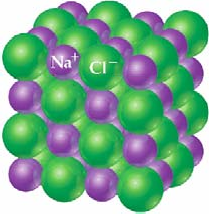
\includegraphics[width=0.5\textwidth]{chapter9/nacl-structure}
	\caption{Structure of Sodium Chloride (\ce{NaCl})}
	\label{fig:nacl-structure}
\end{figure}
In this three-dimensional array of ions, each \ce{Na+} ion is surrounded by siz \ce{Cl-} ions, and each \ce{Cl-} ion is surrounded by six \ce{Na+} ions.

\section{Formation of \ce{NaCl}}\label{sec:formation-of-nacl}
\begin{itemize}
	\item What drives the reaction between \ce{Na (s)} and \ce{Cl2 (g)} to form \ce{NaCl}?
	\item \ce{Na} has a relatively low first \hyperref[sec:ionization-energy]{ionization energy} (i.e., it is perfectly happy to give up its valence electron).
	\emph{Ask yourself, what is the electron configuration of the resulting \ce{Na+} cation}?
	\item \ce{Cl} has a strong tendency to gain an electron, which is manifested in its large negative electron affinity ($E_{a} = -349 \frac{\mbox{kJ}}{\mbox{mol}}$).
	\emph{Ask yourself, what is the electron configuration of the resulting \ce{Cl-} cation}?
	\item In addition, as the \ce{Na+} and \ce{Cl-} ions are drawn together to form \ce{NaCl}, a substantial amount of energy is released, known as the \emph{lattice energy}.
\end{itemize}

\section{Lattice Energy}\label{sec:lattice-energy}
\begin{itemize}
	\item \definition{Lattice energy}{The energy required to completely separate a mole of a solid ionic compound into its gaseous ions.}
	\item Lattice energies are positive as energy is required to overcome attractive forces between oppositely charged ions.
	For example,
	\reaction{NaCl(s) -> Na+(g) + Cl-(g)\ \ \ \ \ \ \ \ \ \Delta H_{lattice} = +788 \frac{\mbox{kJ}}{\mbox{mol}}}
	\item The energy associated with electrostatic interactions is governed by Coulomb's Law:
	\begin{equation}
		E_{el} = \frac{\kappa Q_{1}Q_{2}}{d}
		\label{eq:coulombs-law}
	\end{equation}
	\item Lattice energy increases with the charge on the ions.
	\item It also increases with decreasing size of ions.
	\item See the worked example entitled~\nameref{sec:magnitudes-of-lattice-energies}.
\end{itemize}

\section{Magnitudes of Lattice Energies}\label{sec:magnitudes-of-lattice-energies}
Which substance would you expect to have the greatest lattice energy, \ce{MgF2}, \ce{CaF2}, or \ce{ZrO2}?

\begin{answer}
	\reaction{
		MgF2(s) -> Mg^{2+}(g) + 2F-(g)
	}
	Because the product of the charge, $Q_{1}Q_{2}$, appears in the numerator of the equation above, the lattice energy will increase dramatically when the charges of the ions increase.
	Thus,
	\reaction{
		MgF2 \ \ Q1&=+2 \ \ Q2 &= -1\\
		CaF2 \ \ Q1&=+2 \ \ Q2 &= -1\\
		ZrO2 \ \ Q1&=+4 \ \ Q2 &= -2\\
	}
	\reaction{CaF2 $<$ MgF2 $<$ ZrO2}
\end{answer}

\begin{table}[H]
	\centering
	\caption{Lattice Energies for Some Ionic Compounds}
	\label{tab:lattice-energies-for-ionic-compounds}
	\begin{tabular}{l l|l l}
		\textbf{Compound} & \textbf{Lattice Energy (kJ/mol)} & \textbf{Compound} & \textbf{Lattice Energy (kJ/mol)}\\
		\hline
		\ce{LiF} & 1030 & \ce{MgCl2} & 2326 \\
		\ce{LiCl} & 834 & \ce{SrCl2} & 2127 \\
		\ce{LiI} & 730 & & \\
		\ce{NaF} & 910 & \ce{MgO} & 3795 \\
		\ce{NaCl} & 788 & \ce{CaO} & 3414 \\
		\ce{NaBr} & 732 & \ce{SrO} & 3217 \\
		\ce{NaI} & 682 & & \\
		\ce{KF} & 808 & \ce{ScN} & 7547 \\
		\ce{KFCl} & 701 & & \\
		\ce{KBr} & 671 & & \\
		\ce{CsCl} & 657 & & \\
		\ce{CsI} & 600 & & \\
	\end{tabular}
\end{table}

\section{Covalent Bonding}\label{sec:covalent-bonding}
\begin{minipage}[t]{0.3\textwidth}
	\begin{figure}[H]
		\centering
		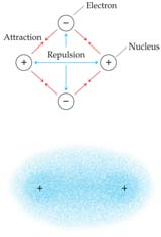
\includegraphics[width=\textwidth]{chapter9/covalent-bonding}
		\caption{Covalent Bonding}
		\label{fig:covalent-bonding}
	\end{figure}
\end{minipage}\hfill%
\begin{minipage}[t]{0.7\textwidth}
	\begin{itemize}
		\item In covalent bonds, atoms share electrons.
		\item There are several electrostatic interactions in these bonds:
		\begin{itemize}
			\item Attractions between electrons and positive nuclei.
			\item Repulsions between electrons
			\item Repulsions between nuclei
			\item Attractive forces must outweigh the repulsive ones
		\end{itemize}
	\end{itemize}
\end{minipage}

\section{Lewis Structures}\label{sec:lewis-structures}
\begin{itemize}
	\item Consider two Hydrogen atoms coming together to form a covalently bonded \ce{H2} molecule:
	\reaction{ \chemfig{\charge{0=\.}{H}} + \chemfig{\charge{180=\.}{H}} -> \chemfig{\charge{0=\:}{H}H}}
	\item The \ce{H2} molecule on the right, with its two electrons, exhibits the noble-gas configuration of Helium.
	The shared pair of electrons can be represented by a single bond, as shown below>
	\reaction{\chemfig{\charge{0=\:}{H}H} = \chemfig{H-H}}
	\item Consider two chlorine atoms coming together to form a covalently bonded \ce{Cl2} molecule:
	\reaction{ \chemfig{\charge{0=\.,90=\:,180=\:,270=\:}{Cl} + \charge{0=\:,90=\:,180=\.,270=\:}{Cl}} -> \chemfig{\charge{0=\:,90=\:,180=\:,270=\:}{Cl}\charge{0=\:,90=\:,270=\:}{Cl}}}
	\item Each chlorine atom on the right now has a \textit{complete octet} of electrons by sharing the bonding electron pair.
	It achieves the noble gas configuration of argon (Ar).
	Again, the shared pair of electrons can be represented by a single bond, as shown below.
\end{itemize}

\section{Typical Bonding Motifs}\label{sec:typical-bonding-motifs}
Typical bonding motifs above: hydrogen and halogens typically form one bond, oxygen two bonds, nitrogen three bonds, and carbon four bonds.
\reaction{
	\chemfig{H-\charge{0=\:,90=\:,270=\:}{F}}\ \ \ \ \ \ \ \
	\chemfig{H-\charge{0=\:,90=\:}{O}(-[:270]H)}\ \ \ \ \ \ \ \
	\chemfig{H-\charge{90=\:}{N}(-[:270]H)-H}\ \ \ \ \ \ \ \
	\chemfig{H-C(-[:90]H)(-[:270]H)-H}
}

\section{Multiple Bonds}\label{sec:multiple-bonds}
\begin{itemize}
	\item Double bonds in \ce{CO2}:
	\reaction{
		\chemfig{\charge{0=\:,90=\.,180=\:,270=\.}{O}} +
		\chemfig{\charge{0=\.,90=\.,180=\.,270=\.}{C}} +
		\chemfig{\charge{0=\:,90=\.,180=\:,270=\.}{O}} ->
		\chemfig{\charge{90=\:,270=\:}{O}=C=\charge{90=\:,270=\:}{O}}
	}
	\item Triple bond in \ce{N2}:
	\reaction{
		\chemfig{\charge{0=\.,90=\.,180=\:,270=\.}{N}} +
		\chemfig{\charge{0=\:,90=\.,180=\.,270=\.}{N}} ->
		\chemfig{\charge{180=\:}{N}~\charge{0=\:}{N}}
	}
\end{itemize}

\section{Bond Polarity and Electronegativity}\label{sec:bond-polarity-and-electronegativity}
\begin{itemize}
	\item Molecules such as \ce{H2}, \ce{N2}, \ce{Cl2}, etc are said to be \textbf{nonpolar}.
	\item \emph{A nonpolar covalent bond} is one in which the electrons are shared equally between two atoms.
	\item On the other hand, \emph{a polar covalent bond} is one in which one of the atoms exerts a greater attraction for the bonding electrons than the other.
	\item In other words, there exists a bond between atoms of different \emph{electronegativities} (e.g., O-H, C-H, N-H, etc.).
\end{itemize}

\section{Electronegativity}\label{sec:electronegativity}
\begin{itemize}
	\item \definition{Electronegativity}{the ability of atoms in a molecule to attract electrons to themselves.}
	\item On the periodic table, electronegativity increases as you go$\dots$
	\begin{itemize}
		\item from left to right across a row
		\item from bottom to the top of a column.
	\end{itemize}
\end{itemize}
\begin{figure}[H]
	\centering
	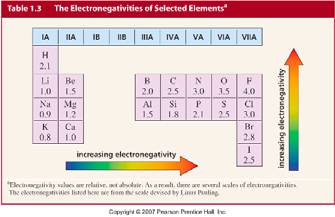
\includegraphics[width=\textwidth]{chapter9/selected-electronegativities}
	\caption{The Electronegativities of Selected Elements}
	\label{fig:selected-electronegativities}
\end{figure}

\section{Polar Covalent Bonds}\label{sec:polar-covalent-bonds}
\begin{itemize}
	\item Though atoms often form compounds by sharing electrons, the electrons are not always shared equally.
	\item Fluorine pulls harder on the electrons it shared with Hydrogen than Hydrogen does.
	\item Therefore, the Fluorine end of the molecule has more electron density than the hydrogen end.
\end{itemize}

\begin{figure}[H]
	\centering
	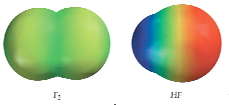
\includegraphics[width=\textwidth]{chapter9/polar-covalent-bonds-examples}
	\caption{Polar Covalent Bonds}
	\label{fig:polar-covalent-bonds}
\end{figure}

\begin{table}[H]
	\centering
	\caption{Electronegativity and Bond Polarity}
	\label{tab:electronegativity}
	\begin{tabular}{|*{4}{c|}}
		\hline
		\textbf{Compound} & \textbf{\ce{F2}} & \textbf{\ce{HF}} & \textbf{\ce{LiF}}\\
		\hline
		Electronegativity & 4.0 - 4.0 = 0 & 4.0 - 2.1 = 1.9 & 4.0 - 1.0 = 3.0\\
		\hline
		Type of bond & Nonpolar covalent & Polar covalent & Ionic\\
		\hline
	\end{tabular}
\end{table}

\begin{itemize}
	\item When two atoms share electrons unequally, a \emph{bond dipole} results.
	\item The \emph{dipole moment}, $\mu$, produced by two equal but opposite charges separated by a distance $r$ is calculated as:
	\begin{equation}
		\mu = Qr
		\label{eq:dipole-moment}
	\end{equation}
	\item The dipole is measured in debye (D) units.
\end{itemize}
\begin{figure}[H]
	\centering
	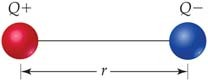
\includegraphics[width=\textwidth]{chapter9/dipole-moment}
	\caption{Dipole Moment $\mu$}
	\label{fig:dipole-moment}
\end{figure}

\begin{table}[H]
    \centering
    \begin{threeparttable}
		\caption{Polar Covalent Bonds}
		\label{tab:polar-covalent-bonds}
		\begin{tabular}{p{0.2\textwidth} p{0.22\textwidth} p{0.22\textwidth} p{0.25\textwidth}}
			\textbf{Compound} & \textbf{Bond Length (\si{\angstrom})} & \textbf{Electronegativity} & \textbf{Dipole Moment (D)}\\
			\hline
			\ce{HF}  & 0.92 & 1.9 & 1.82\\
			\ce{HCl} & 1.27 & 0.9 & 1.08\\
			\ce{HBr} & 1.41 & 0.7 & 0.82\\
			\ce{HI}  & 1.61 & 0.4 & 0.44\\
			\hline
		\end{tabular}
		\begin{tablenotes}
			\small
			\item The greater the difference in electronegativity, the more polar the bond is.
		\end{tablenotes}
	\end{threeparttable}
\end{table}


\section{Writing Lewis Structures}\label{sec:writing-lewis-structures}
\reaction{
	\chemfig{H-H}\ \ \ \ \ \ \ \ \ \ \ \ \
	\chemfig{\charge{90=\:,180=\:,270=\:}{Cl}-\charge{0=\:,90=\:,270=\:}{Cl}}
}
\begin{itemize}
	\item Lewis structures are representations of molecules showing all electrons, bonding and nonbonding.
\end{itemize}

\begin{enumerate}
	\item Find the sum of valence electrons of all atoms in the polyatomic ion or molecule.
	\begin{itemize}
		\item If it is an anion, add one electron for each negative charge.
		\item If it is a cation, subtract one electron for each positive charge.
		\item \textcolor{red}{Total number of valence electrons for \ce{PCl3} is:\_\_\_\_ \begin{answer}5 + (7*3) = 26\end{answer}}
	\end{itemize}
	\item The central atom is the \emph{least} electronegative element that isn't Hydrogen.
	Connect the other atoms to it by single bonds.
	\item Fill the octets of the outer atoms.
	\begin{itemize}
		\item \textcolor{red}{How many electrons have you accounted for in the above structure?} \begin{answer}24\end{answer}
		\item \textcolor{red}{How many do you have left?} \begin{answer}2\end{answer}
		\item Fill in the octet of the central atom.
		\item If you run out of electrons before the central atom has an octet: form multiple bonds until it does
		\reaction{\chemfig{H-C-\charge{0=\:,90=\:,270=\:}{N}} -> \chemfig{H-C~\charge{0=\:}{N}}}
	\end{itemize}
\end{enumerate}

\begin{itemize}
	\item \emph{Then assign formal charges}.
	\item For each atom, count the electrons in lone pairs and half the electrons it shares with other atoms.
	\item Subtract that from the number of valence electrons for that atom: the difference is its formal charge (see~\eqref{eq:formal-charge}).
\end{itemize}

\begin{equation}
	\mbox{formal charge} = \mbox{\# of valence electrons} - \mbox{\# of lone-pair electrons} - \frac{1}{2}\mbox{ \# of bonding electrons}
	\label{eq:formal-charge}
\end{equation}

\begin{figure}[H]
	\centering
	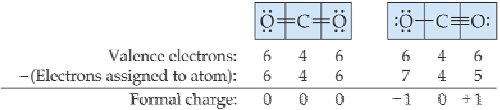
\includegraphics[width=\textwidth]{chapter9/formal-charges}
	\caption{Formal Charges for \ce{CO2}}.
	\label{fig:formal-charges}
\end{figure}

\begin{itemize}
	\item The best Lewis structure$\dots$
	\begin{itemize}
		\item $\dots$ is the one with the fewest charges.
		\item $\dots$ puts a negative charge on the most electronegative atom.
	\end{itemize}
\end{itemize}

\begin{figure}[H]
	\centering
	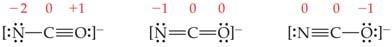
\includegraphics[width=\textwidth]{chapter9/formal-charges-2}
	\caption{Choosing the best formal charge for \ce{CON}.}
	\label{fig:formal-charges-2}
\end{figure}



\section{Lewis Structures for Polyatomic Ions}\label{sec:lewis-structures-for-polyatomic-ions}
Draw the Lewis structures for:
\begin{enumerate}[label=(\alph*)]
	\item \ce{ClO2-}
	\begin{answer}
		7 + 2(6) + 1 = 20 valence electrons
		\reaction{\chemfig{
		% FIXME: Figure out why the compiler doesn't like the chemleft and chemright being here
%			\chemleft{[}
			\charge{90=\:,180=\:,270=\:}{O}-
			\charge{90=\:,270=\:}{Cl}-
			\charge{0=\:,90=\:,270=\:}{O}
%			\chemright{]}^{-}
		}}
	\end{answer}
	\item \ce{SO4^2-}
	\begin{answer}
		6 + 4(6) + 2 = 32 valence electrons
		\reaction{\chemfig{\charge{90=\:,180=\:,270=\:}{O}-S(-[:90]\charge{0=\:,90=\:,180=\:}{O})(-[:270]\charge{0=\:,180=\:,270=\:}{O})-\charge{0=\:,90=\:,270=\:}{O}}}
	\end{answer}
	\item \ce{CO3^2-}
	\begin{answer}
		4 + 3(6) + 2 = 24 valence electrons
		\begin{equation*}
			\chemfig{([:30]\charge{135=\:,225=\:,315=\:}{O}-) C (=[:90]\charge{45=\:,135=\:}{O})(-[:-30]\charge{45=\:,225=\:,315=\:}{O})} \hfill\ \ \ \ \ \ \ \ \ \ \ \ \ \
			\chemfig{([:30]\charge{135=\:,315=\:}{O}=) C (-[:90]\charge{0=\:,90=\:,180=\:}{O})(-[:-30]\charge{45=\:,225=\:,315=\:}{O})} \hfill\ \ \ \ \ \ \ \ \ \ \ \ \ \
			\chemfig{([:30]\charge{135=\:,225=\:,315=\:}{O}-) C (-[:90]\charge{0=\:,90=\:,180=\:}{O})(=[:-30]\charge{45=\:,225=\:}{O})}
		\end{equation*}
	\end{answer}
\end{enumerate}

\section{Resonance}\label{sec:resonance}
\begin{itemize}
	\item One possible Lewis structure of the ozone (\ce{O3}) molecule is depicted below.
	\reaction{\chemfig{([:30]\charge{135=\:,225=\:,315=\:}{O}-) \charge{90=\:}{O} (=[:30]\charge{0=\:,90=\:,180=\:}{O})}}
	\item But this is not consistent with the observed structure of ozone, whereby$\dots$
	\begin{itemize}
		\item both $\ce{O-O}$ bonds are the same length.
	\end{itemize}
	\item One Lewis structure cannot accurately describe a molecule like ozone.
	\item We use multiple structures (i.e. \emph{resonance structures}) to describe the molecule.
	\item Placement of atoms remain the same, but the placement of electrons are different.
	\item A double headed arrow is used to indicate that the real molecule is described by an average of the resonance structures.
\end{itemize}

\subsection{An Analogy to Color Mixing}\label{subsec:an-analogy-to-color-mixing}
Just as green is a \textit{blend} of blue and yellow$\dots$ the real structure of ozone is a \textit{blend} of the two resonance structures.

\section{Exceptions to the Octet Rule}\label{sec:exceptions-to-the-octet-rule}
\begin{itemize}
	\item The three types of systems that don't follow the octet rule are as follows:
	\begin{itemize}
		\item Ions or molecules with an odd number of electrons
		\item Ions or molecules with less than an octet
		\item Ions or molecules with more than eight valence electrons (an expanded octet)
	\end{itemize}
\end{itemize}

\subsection{Odd Number of Electrons}\label{subsec:odd-number-of-electrons}
Ions and molecules with an odd number of electrons (e.g., \ce{ClO2}, \ce{NO}, \ce{NO2}, and \ce{O2}).

\begin{equation*}
\begin{aligned}
	\chemfig{\charge{90=\:,270=\.}{\ce{N}}=\charge{90=\:,270=\:}{\ce{O}}} \mbox{  and  } \chemfig{\charge{90=\:,270=\:}{\ce{N}}=\charge{90=\:,270=\.}{\ce{O}}}
\end{aligned}
\end{equation*}

\subsection{Fewer than Eight Electrons}\label{subsec:fewer-than-eight-electrons}
\reaction{\chemfig{([:30]\charge{135=\:,225=\:,315=\:}{F}-)B(-[:90]\charge{0=\:,90=\:,180=\:}{F})(-[:-30]\charge{45=\:,225=\:,315=\:}{F})}}
\begin{itemize}
	\item Consider \ce{BF3}
	\begin{itemize}
		\item Notice how the central boron does not have a complete octet?
		\item What about resonance?
		\item See worked example below:
	\end{itemize}
\end{itemize}

Draw the Lewis structure for boron trifluoride, \ce{BF3}, and explain why it does not obey the octet rule.

\begin{answer}
	These resonance structures are less important than the first because they put positive charge on the most electronegative fluorine atoms!
\end{answer}

\subsection{More than Eight Electrons}\label{subsec:more-than-eight-electrons}
\begin{itemize}
	\item The only way \ce{PCl5} can exist is if phosphorus has 10 valence electrons around it.
	\item It is allowed to expand the octet of atoms on or below the 3rd row/period.
	\item \emph{Ask yourself, does \ce{NCl5} exist?} \begin{answer}No.\end{answer}
	\item Most likely the $d$ orbitals in these atoms participate in bonding.
\end{itemize}

\section{Covalent Bond Strength}\label{sec:covalent-bond-strength}
\reaction{\chemfig{\charge{90=\:,180=\:,270=\:}{Cl}-\charge{0=\:,90=\:,270=\:}{Cl}}(g) -> 2\charge{0=\.,90=\:,180=\:,270=\:}{Cl}(g)}
\begin{itemize}
	\item The strength of a bond is measured by determining how much energy is required to break the bond.
	\item This is the \emph{bond enthalpy}.
	\item The bond enthalpy for a \ce{Cl}-\ce{Cl} bond is measured to be 242 kJ/mol.
\end{itemize}

%</Chapter-9>
\end{document}
